\chapter[Surrogate ML Model Development]{A surrogate machine learning model for advanced gas-cooled reactor graphite core safety analysis}


\label{cha:surrogate}


This chapter is adapted from the academic article \textit{A surrogate machine learning model for advanced gas-cooled reactor graphite core safety analysis} published in the journal of Nuclear Engineering and Design \cite{jones2022surrogate}. It details the development of a machine learning model intended to surrogate the functions of the traditional engineering model Parmec \cite{wiki:xxx} used for advanced gas-cooled reactor safety analysis.

\section{Abstract}

A surrogate machine learning model was developed with the aim of predicting seismic graphite core displacements from crack configurations for the advanced gas-cooled reactor. The model was trained on a dataset
generated by a software package which simulates the behaviour of the graphite core during a severe earthquake.
Several machine learning techniques, such as the use of convolutional neural networks, were identified as highly
applicable to this particular problem. Through the development of the model, several observations and insights
were garnered which may be of interest from a graphite core analysis and safety perspective. The best performing
model was capable of making 95\% of test set predictions within a 20 percentage point margin of the ground
truth.

\section{Research Highlights}

There were three main highlights to this research article:

\begin{enumerate}
	
\item A surrogate machine learning model was developed
which aims to predict seismic graphite core displacements from crack configurations for the advanced gas-cooled reactor. The model was trained on a dataset generated by a software package which simulates the behaviour of the graphite core during a severe earthquake.
The main motivation behind this research was to increase the computational efficiency of seismic displacement output data generation in order to allow a wider
search of the vast problem space. 

\item Following the training process of the models, the generation of output values takes less than one second. Using the same hardware, the equivalent data generation time would be over
2 hours using the original Parmec software.
The best performing model was capable of making
95\% of test set predictions within a 20 percentage point
margin of the ground truth. 

\item Through a process of feature selection i.e. reducing the expression of certain parts of the data space, engineering insights into the underlying nature of the dataset and problem can be inferred. For example, optimal model performance was observed when including input information from only the top three levels of the graphite core. From this, we can conclude that information regarding the bottom of the graphite core may be irrelevant to the prediction of displacement outputs. The feature selections identified not only are useful in the production of machine learning models, but may also be useful in a wider context i.e. engineering safety analysis in this field.


\end{enumerate}


\section{Introduction and Background}

Much of what is contained in the introductory and background sections of the journal article discussed here has already been covered in this thesis. Rather than repeat this information, the relevant sections shall simply be referred to here.

\begin{enumerate}
	
	\item Information concerning the underlying engineering problem, the advanced gas-cooled reactor (AGR) and the traditional engineering model Parmec used to perform safety analysis for the AGR is discussed in chapter~\ref{cha:engineering}.
	
	\item Regarding background information on the workings of machine learning methods, models and concepts is available in chapter~\ref{cha:ML}.
	
	\item A discussion and exploration of the dataset is given in chapter~\ref{cha:dataset}, with the programmatic framework developed to create datasets and streamline machine learning model production detailed in section~\ref{framework}.
	
	
	
\end{enumerate}

\section{Data Selection and Focus} \label{data_selection}

As explained in subsection~\ref{data:outputs}, each Parmec case contains approximately 6.8 million output parameters. For the purpose of this work,  this large data space was narrowed down into a usable format. The process of data selection was informed by the preliminary experiments reported in Chapter~\ref{cha:preliminary} and the data visualisation process from section~\ref{data:visualisation} .  
\\

\noindent
Of the six output metrics, a single displacement metric was chosen (displacement translation along the horizontal axis in the direction of the applied earthquake acceleration) at a single time frame (time frame 48 - approximately 3.8 seconds into the simulated earthquake). The justification for this selection is made at the start of section~\ref{prelim:whole} and can be summarised by examining Figure~\ref{fig:earthquake}. It can be seen that the earthquake is well underway at this point and the data from later time-steps was found to have a greater level of homogeneity and less variation between instances.
\\

\noindent
The output space was further narrowed to include data for just a single brick at a time i.e. a single label value for each instance. The selection of outputs allows the research problem to be expressed as single label regression (as opposed to multi label regression where we would attempt to predict multiple outputs per instance). The decision to focus on only a single brick and not outputs for the whole go was again made based on the findings of the preliminary experiment detailed in section~\ref{prelim:whole} where unsatisfactory results were achieved from training a model to predict outputs for all interstitial bricks. It was also discussed in subsection~\ref{correlation} that outputs for interstitial bricks poorly correlate with each other, particularly when the bricks are from geographically remote parts of the core.
\\

\noindent
The brick chosen was the one located at the upper most level at the centre of the core. This position of this brick is shown in the lower part of Figure~\ref{fig:pos_distr}. This brick is at a particularly important position from an engineering perspective. On average, the closer a channel is to the centre of the core, the higher its translational displacement relative to the surrounding structure (see Figure~\ref{fig:composite} from subsection~\ref{data:entire}). The upper level may also be considered of greater importance than those lower down, as it is the initial point of entry for a control rod. The decision to choose this brick was also informed by literature concerning engineering assessments of the AGR (see section~\ref{engineering:literature}).
\\

\noindent
The distribution of horizontal displacement at time frame 48 for all ~8300 instances is shown as a histogram in the upper part of Figure~\ref{fig:pos_distr}. It can be seen that the labels take the form of a Gaussian distribution, but with the modal value to the left of the median and mode. The data also has a long tail on the right hand side i.e. there are a number of outliers on the upper end of the distribution.

\begin{figure*}[p]
	\centering
	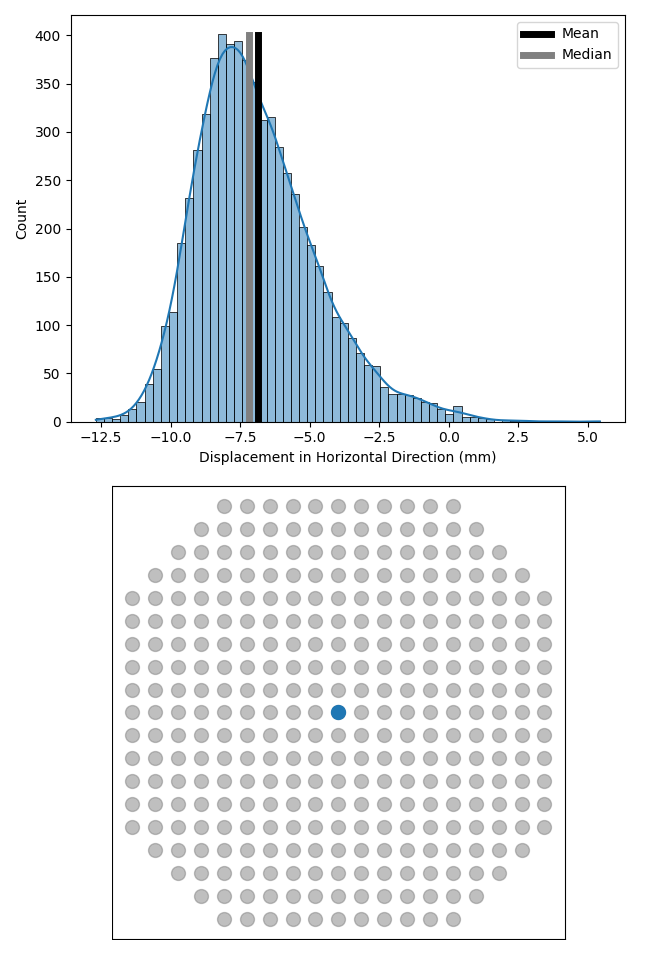
\includegraphics[scale=0.7]{Figures/position_distribution.png}
	\caption{The Position in the core from which the labels are representative of (\textbf{Bottom}); Distribution of ~8300 values in the label set (\textbf{Top})}
	\label{fig:pos_distr}
\end{figure*}

\section{Surrogate Model Development and Design} \label{method}

\subsection{Traditional Methods} \label{traditional}

We began with the use of traditional machine learning models, otherwise known as shallow methods. The methods used included: linear regression, Huber regression, support vector machines \cite{smola2004tutorial} and decision tree regression \cite{navada2011overview}. Each model type was optimised using the training set (N) followed by evaluation against the test set ($N_t$). 

\subsection{Neural Networks}

The remainder of this section discusses the development of experiments involving neural networks. Two types of neural network architecture were employed: dense neural networks (also known as fully connected networks) and convolutional neural networks.
\\

\noindent
To this end, each experimental configuration of parameters was evaluated by training a model using 10-fold cross-validation \cite{refaeilzadeh2009cross}. To account for the stochastic nature of model training caused by the random initialisation of model weights, the training process was repeated 32 for each cross-validation fold. At the start of training, a learning rate of 5.00E-04 was employed, with this being programmatically halved each time a performance plateau is detected (no validation loss improvement for 50 epochs). Early stopping \cite{yao2007early} was used when the learning rate drops below  1.00E-05, with training terminated and the parameters retained from the point at which lowest validation loss was achieved. Each optimised model was then evaluated against the test set of 2000 samples. A graphical representation of this process is seen in Figure~\ref{fig:train_history}. 
\\

\noindent
The next subsection discusses the general process of hyper-parameter optimisation during model design. The subsection after that discusses differing data input encoding shapes and the model architectures they require. Finally in this section, we discuss the impact of feature selection i.e. reducing the input feature space provided to the model.

\begin{figure}[h]
	\centering
	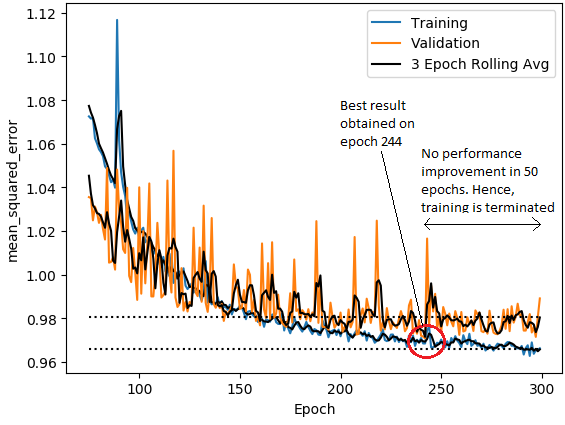
\includegraphics[scale=0.55]{Figures/Training History.png}
	\caption{Example of Model Training and Validation with Early Stopping and Model Saving} {As can be seen, the best model performance is produced on epoch 244 where a validation loss of 0.97 is obtained. After training for another 50 epochs, training is terminated, as in this case minimum training rate has already been achieved. The optimal model weights are then retained to evaluate against the test set.}
	\label{fig:train_history}
\end{figure}

\subsection{General Hyper-Parameters}

As mentioned in subsection~\ref{NN}, several hyper-parameters must be chosen for a neural network. The optimal selection of hyper-parameters were chosen through an experimental processes. 
\\

\noindent
The first parameter that was chosen was the optimiser. After evaluating several optimiser algorithms, including the RMSprop, Adagrad, and SGD configurations, the Adam optimiser with Nesterov momentum \cite{dozat2016incorporating} was was chosen as it provided the best model performance.
\\

\noindent
Three model additional model hyper-parameters were also refined: nodal architecture, activation functions and regularisation. Starting with the architecture, this was developed through a trial and error method. Beginning with a simple structure of a single hidden layer with a width of four nodes, this was then expanded and adjusted experimentally, using the testing loss for each configuration as a measure of its performance. Guidance was taken from previous works as to what architectures may be most effective, including \cite{fernandez2017nuclear} which describes four distinct architectures which were used as a starting point for the experiments performed here. 
\\

\noindent
In tandem with the nodal architecture, the use of activation functions were chosen experimentally. At first, the same activation function was applied to each layer (bar the output layer). The use of three commonly employed activation functions were tested: sigmoid, the rectified linear unit (ReLu) \cite{hara2015analysis} and the hyperbolic tangent function \cite{kalman1992tanh}. Also tested was the less common softplus function \cite{zheng2015improving} which has been used in other surrogate model works, including \cite{liang2018deep}. In addition to a model design that uses the same activation function in all layers, alternative configurations were tested . Initially, a method employing non-linear activations on every other layer was employed, with the alternating layers simply outputting the linear combination of inputs and weights. Inspiration for this approach was taken from \cite{ahn2020deep} where non-linear activations were only placed on every 4th layer of the neural network architecture. This was further modified to an architecture employing two different non-linear activation functions in the same model, with the greatest success being observed when alternating softmax and tanh. The final model, demonstrating the optimal architecture, is shown in Figure~\ref{fig:model_architecture}.
\\

\noindent
The regularisation parameter was also optimised experimentally. The most effective technique was found to be dropout \cite{srivastava2014dropout} where the output of randomly selected layers are negated. It was determined experimentally that a dropout parameter of 0.4 was optimal - the output of 40\% of the nodes in each layer were randomly dropped. 
\\

\noindent
The experimental models were trained using several loss functions. These were mean squared error (MSE) mean absolute error (MAE) and the Huber loss \cite{huber1964robust}. By inter-comparing each loss function, it was found that Huber was the optimal loss function for training the model.


\begin{figure*}[h]
	\centering
	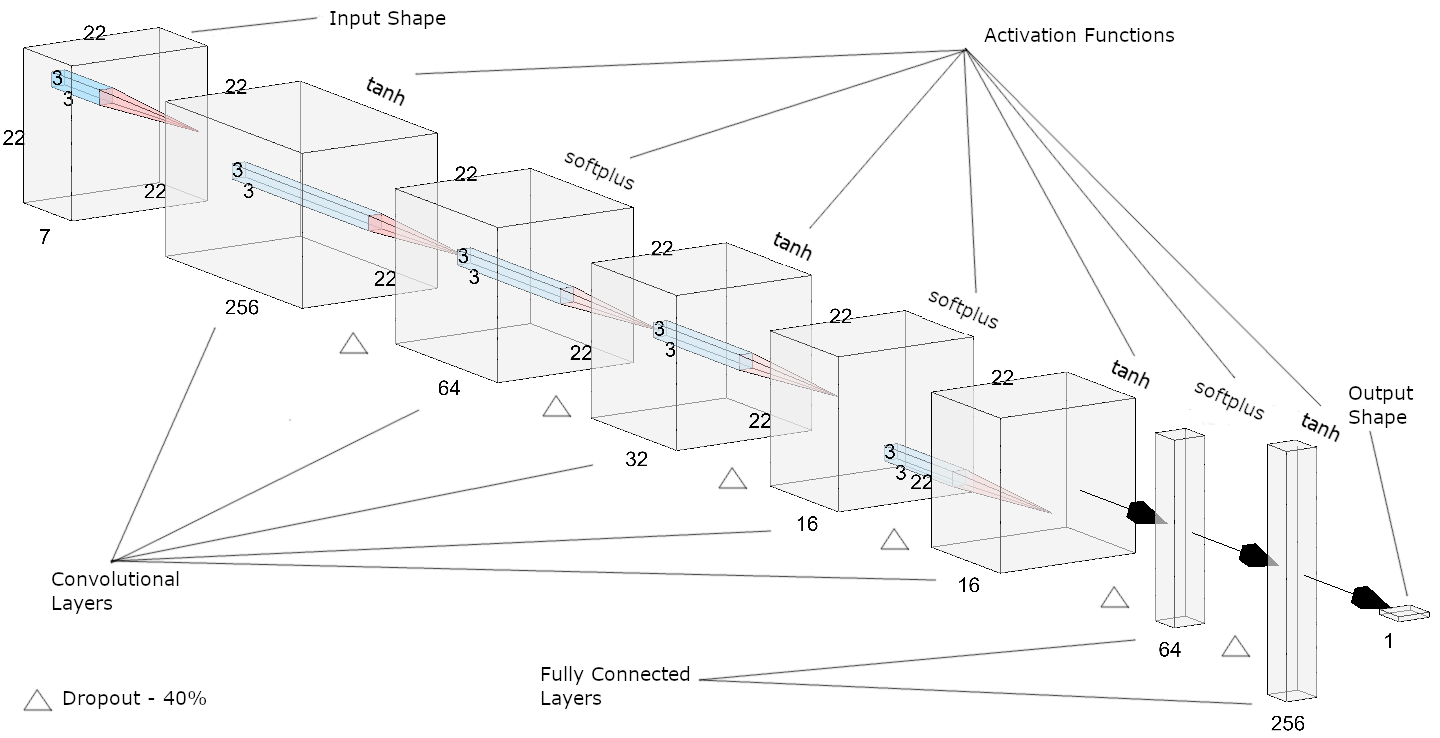
\includegraphics[scale=1.2]{Figures/architecture_final.png}
	\caption{The Final Architecture of the Model}
	\label{fig:model_architecture}
\end{figure*} 

\begin{figure*}[p]
	\centering
	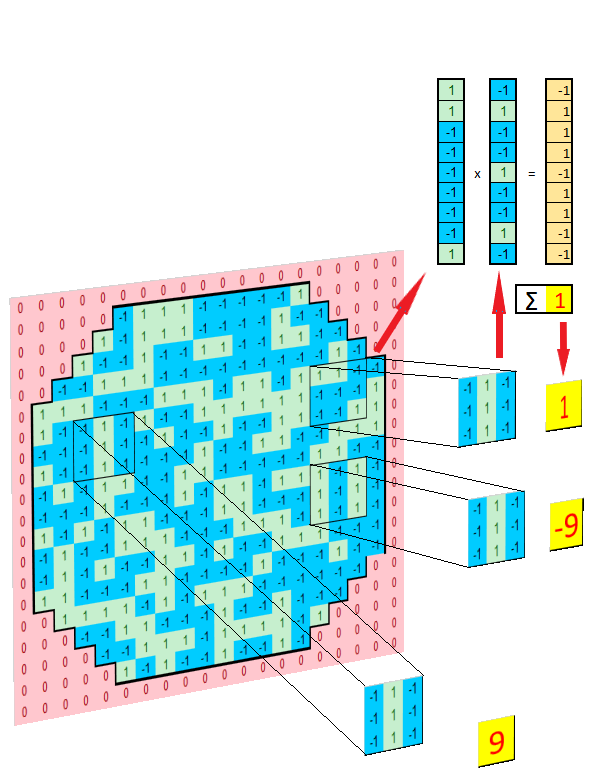
\includegraphics[scale=0.8]{Figures/convo_proj2.png}
	\caption{Convolution on a 2-dimensional Input Space Using a 3x3 Filter} {The input space is a top-down cross-sectional slice of a 3-dimensional tensor. This represents the distribution of cracks in a single level of the AGR reactor for a single example. The corners and edges have been padded with zeros to maintain a regular shape. The convolutional operation has been performed at select locations. \textbf{Lower-right}: the patch from the input space is the perfect inverse of the filter, resulting in the lowest possible output value (-9). \textbf{Left}: the input patch is a perfect match of the filter, resulting in the maximum output (9). \textbf{Top-right}: a middling example where the input patch has only a slight resemblance to the filter. Outside of the image on the top right-right hand corner, the mathematical operation between a data patch and filter is seen: both are flattened into a vector followed by a dot product calculation. }
	\label{fig:convo_operation}
\end{figure*} 

\begin{figure*}[p]
	\centering
	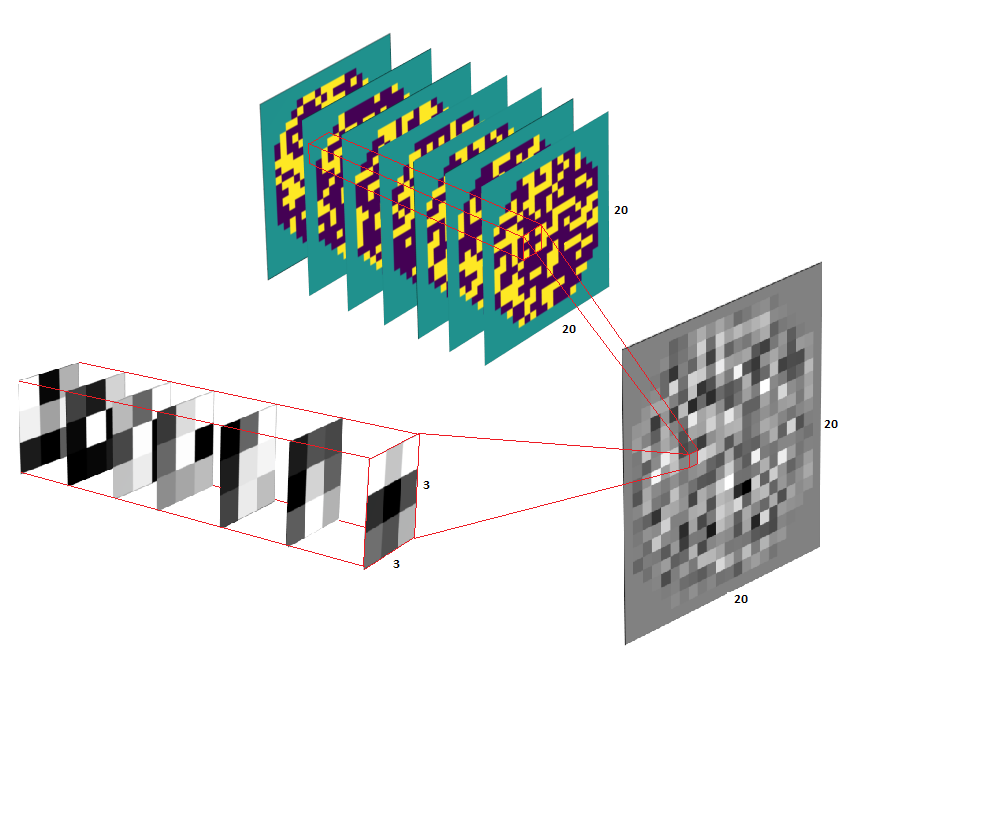
\includegraphics[scale=0.7]{Figures/convo_vis.png}
	\caption{Convolution on a Single Instance Encoded in a 3-dimensional Format Using an Example Multi Channel Filter} {\textbf{Top}: a single instance encoded with each core level represented as a separate channel. \textbf{Left}: a single filter from the first layer of a CNN, the planar dimensions are smaller than the input space (3x3), but the number of channels are equal to the number in the input space (7). The filter performs the mathematical operation shown in Figure~\ref{fig:convo_operation} on each channel. The sum of all channels operations forms a single value in the output feature map for this filter. \textbf{Right}: the feature map for the filter. If the aforementioned mathematical operation is performed across the entire input space, we get the feature map shown here. If this process is performed for multiple filters, several feature maps are produced, which each represent channel inputs for the next convolutional layer. Alternatively, the feature map can be flattened as to form the input for a dense layer). }
	\label{fig:feature_maps}
\end{figure*}


\newpage
\subsection{Neural Network Input Encoding} \label{encoding_method}

Three alternative configurations of neural network were employed, each requiring a differing data encoding format, as outlined in the following subsections. One of these configurations employs only dense neural network architecture, with the other two employing convolutional neural network architecture.  An experiment was designed to compare each of these encoding formats in turn.
\\

\noindent
In each case, the number of input features is the same: 1988 (the number of fuel bricks). Similarly, there is a single output (the displacement for the central interstitial brick in the top level). In each case, a similar model architecture is used, with notable exceptions such as the use of only dense layers or the inclusion of convolutional layers.

\begin{table}[h!]
	\begin{center}
		
		\begin{tabular}{c|c|c|r|c} % <-- Alignments: 1st column left, 2nd middle and 3rd right, with vertical lines in between
			\textbf{Encoding} & \textbf{Input} & \textbf{Output} & \textbf{Model} \\
			
			\textbf{Mode} & \textbf{Format} & \textbf{Shape} & \textbf{Architecture} \\
			\hline
			1D & 1988 & 1 & DNN Only \\
			2D & 7 x 284 &  1 & CNN \& DNN \\
			3D & 7 x 20 x 20 &  1 & CNN \& DNN \\
			
		\end{tabular}
		\caption{Summary of the Input Encoding Experiment} {For each encoding format, the total size of the input is the same; only the shape changes. Additionally, the output label in each case is the same shape. Note also that the 1D encoding requires a model containing only dense layers, whereas 2D and 3D encoding warrants a mix of convolutional and dense layers. }
		\label{tab:encodings}
	\end{center}
\end{table}

\subsubsection{DNN - 1D}

A dense neural network with 1D encoding is employed. In this configuration, the data is encoded in the base format as mentioned in subsection~\ref{data:inputs} where each instance is input to the model as a vector. In the DNN, the output of each layer is fed into all nodes of the subsequent layer.

\subsubsection{CNN - 2D}

A convolutional neural network architecture with 2D encoding. In this format a 2-dimensional filter is applied at select patches on a 2-dimensional input space (Figure~\ref{fig:convo_operation}). To facilitate this, the 1988 element long input feature vector is reshaped into a matrix. The dimensions of this matrix are 7 by 284: the bricks per fuel channel (BFC) by number of fuel channels (NFC), respectively. Hence, in this encoding format, an individual instance has a feature matrix of the form $\textbf{x}_i~=~\{-1, 1\}^{BFC \times NFC}$. This format is analogous to CNNs used for image recognition which use a grey-scale bitmap as input \cite{bui2016using}. 
\\

\noindent
The architecture produced during the DNN optimisation was kept the same. However, the first 5 layers now became CNN layers with the latter two remaining fully connected layers. This resulted in an additional parameter to be optimised: the size of the convolutional window shape (or kernel). A window size of 3 by 3 was experimentally found to produce the best result.

\subsubsection{CNN - 3D} A convolutional neural network architecture with 3D encoding. This arrangement reflects the true positional relationship within the actual core. The bricks are stacked in 7 levels (BFC). At its widest width and breadth, the core is 18 channels across. The tensor has been padded at the edges and corners with zeros to make it a regular shape and keep the input shape the same size in subsequent layers \cite{dwarampudi2019effects}. Consequently, CW \& CB both have a value of 22 due to a double layer of zeros on each side. Therefore the dimensions of this input tensor are bricks per fuel channel (BFC) by core width (CW) by core breadth (CB): 7 by 20 by 20 i.e the input features for each instance is in the form $ \textbf{x}_i~=~\{-1, 0, 1\}^{BFC \times CW \times CB}$. This input shape can again be used by a CNN with a 2-dimensional architecture. However, with a 3-dimensional encoding each core level is used as a separate input channel. In this format, the filter has multiple channels, one for each of the channels in the input space (see Figure~\ref{fig:feature_maps}). This is analogous to CNNs used for image recognition where colour data (usually red, green and blue) are represented by different input channels \cite{albawi2017understanding}. 

\subsection{Feature Selection} \label{feature_selection}

In section~\ref{data}, it is mentioned that the input to Parmec is a vector 1988 elements long, each representing the cracking status on one bricks in the model. So far in this section, we have discussed various dimensional encoding formats available, including a 3-dimensional encoding which represents the true physical arrangement of the core. We have the choice to provide this information to the model in its entirety, or to reduce the scope of these inputs in some way. Through a process of feature selection \cite{gurney1997introduction}, we can actively chose only the most relevant features to the predicted output by monitoring the model performance as the scope is adjusted. Beyond model performance optimisation, the process of feature selection allows insights into the data, including relationships between inputs and outputs, what information is relevant and so on. As mentioned in subsection~\ref{framework}, the framework developed for this research work allows the selection of features programmatically. 
\\

\noindent
The proposed method for feature selection is to split the core in different ways and then perform experiments using only those features. Two differing strategies are discussed in the following sections.

\subsubsection{Regional Selection} \label{regional_selection}

The core features are split into concentric sections as shown in Figure~\ref{fig:regions}.  Recall that the value we aim to predict is for the central channel (Figure~\ref{fig:pos_distr}). Hence each concentric region is effectively further removed from the position of interest. It can be hypothesised that the data for regions closer to the central position are most important to model performance, with importance falling as we move further away. Testing this hypothesis is the purpose for this experiment.
\\

\noindent
Starting with the greater core region (i.e. the whole feature set) a model is trained and evaluated.The feature set is then reduced by incrementally removing channel regions and then training a new model using it. By repeating this process until only the inner channel region remains and evaluating the trained model at each stage, we can choose the optimal features for inclusion.

\begin{figure}[h]
	\centering
	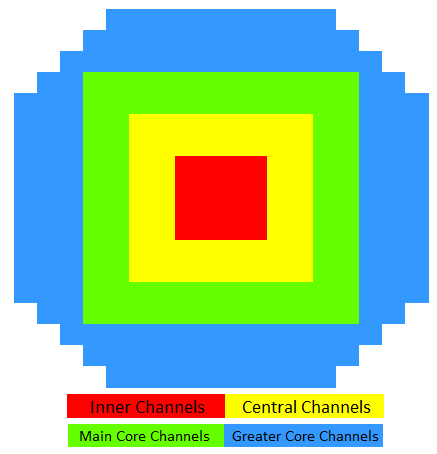
\includegraphics[scale=0.7]{Figures/core_regions.png}
	\caption{The Core Separated into Regions for the Purpose of Feature Selection} {The method of this experiment is discussed in Subsection~\ref{regional_selection} with the results given in Table~\ref{tab:regional}. }
	\label{fig:regions}
\end{figure}

\subsubsection{Level Selection} \label{level_selection}

In addition to feature selection based on the core regions from, the feature set was also varied in size by varying the number of core levels (refer back to Figure~\ref{fig:schematic}). Recall from section~\ref{data_selection} that the brick for which we are attempting to predict displacement values for is in the top layer. Similar to the experiment in the previous subsection, is can be conjectured that the lower levels of the core are less important than those near the top (closer to the point of interest). This again was determined experimentally. Starting with the lowest level (level 1), data for incrementally higher core levels was removed from the feature set, training and evaluating the model each time. 



\section{Results} \label{results}

\subsection{Traditional Methods}

As mentioned in subsection~\ref{traditional}, the experimental processes for this work began with the use of traditional machine learning methods. The results are summarised in Table~\ref{tab:traditional}. As can be seen, the linear regression method produces the best test loss and therefore best performing model. This is followed by the Huber and support vector regression methods. A decision tree regression model can fit the the training data almost perfectly (a training loss of zero). However, the decision tree regression model also performs worst on the testing set, suggesting overfitting.  

\begin{table}[h!]
	\begin{center}
		
		\begin{tabular}{c|c|c|r|c} % <-- Alignments: 1st column left, 2nd middle and 3rd right, with vertical lines in between
			\textbf{Inclusive} & \textbf{Training} & \textbf{Test} \\
			
			\textbf{Levels} & \textbf{Loss} & \textbf{Loss} \\
			\hline
			Linear Regression & 7.2e-3 & 1.2e-2 \\
			Huber Regression & 7.7e-3 &  1.3e-2 \\
			Support Vector Regression & 5.8e-3 &  1.4e-2 \\
			Decision Tree Regression & 0 & 4.7e-2 \\
		\end{tabular}
		\caption{Summary of the Test Results from the Traditional Methods Experiment (Subsection~\ref{traditional})} {Values are in mean squared error (MSE). }
		\label{tab:traditional}
	\end{center}
\end{table}


\subsection{Input Encoding} \label{encoding_results}

Table~\ref{tab:encoding} summarises the results of the experiment outlined in subsection~\ref{encoding_method}, with the best result achieved with each encoding format shown. \\

\begin{table}[h!]
	\begin{center}
		
		\begin{tabular}{c|c|c|r|c} % <-- Alignments: 1st column left, 2nd middle and 3rd right, with vertical lines in between
			\textbf{Encoding} & \textbf{Lowest} & \textbf{Mean} \\
			
			\textbf{Format} & \textbf{Loss} & \textbf{Loss} \\
			\hline
			3D (CNN) & 9.9e-3  & 1.3e-2 \\
			2D (CNN) & 1.1e-2  & 1.6e-2 \\
			1D (DNN) & 1.3e-2 & 1.3e-2 \\
		\end{tabular}
		\caption{Summary of the Test Results from the Input Encoding Experiment (Subsection~\ref{encoding_method})} {Values are in mean squared error (MSE). Each part of the experiment was repeated 32 times for each cross validation fold (320 total) with starting weights initialised randomly each time. The weights were stored at the optimal point during training (lowest validation loss). Each saved model was then evaluated against the test set of 2000 samples, with the lowest and mean values reported in this table.}
		\label{tab:encoding}
	\end{center}
\end{table}

\noindent
From the results, it can be seen that a CNN employing 3D data encoding produces the best performance. In turn, it can also be seen that a CNN employing 2D encoding produces a lower overall loss value than a DNN employing 1D encoding. See subsection~\ref{analysis} for further discussion of these results. 

\subsection{Feature Selection} \label{feature_extract_results}

Recall from subsection~\ref{feature_selection} that two strategies are proposed for experimental feature selection: regional and level selection. 
\\

\noindent
Table~\ref{tab:regional} summarises the results for the regional feature selection experiment (subsection~\ref{regional_selection}). Each row represents a model trained using the data for channels inclusively within the region indicated. For example, Main Core (green in Figure~\ref{fig:regions}) includes data for itself and the regions internal to it (central and inner) but not the region beyond it (greater core). 
\\

\begin{table}[h!]
	\begin{center}
		
		\begin{tabular}{c|c|c|r|c} % <-- Alignments: 1st column left, 2nd middle and 3rd right, with vertical lines in between
			\textbf{Inclusive} & \textbf{Lowest} & \textbf{Mean} \\
			
			\textbf{Regions} & \textbf{Loss} & \textbf{Loss} \\
			\hline
			Greater Core (blue) & 9.9e-3  & 1.3e-2 \\
			Main Core (green) & 1.6e-2 & 1.7e-2 \\
			Central (yellow) & 2.0e-2 & 2.2e-2  \\
			Inner (red) & 2.1e-2 & 2.3e-2  \\
		\end{tabular}
		\caption{Summary of the Test Results from the Regional Feature Selection Experiment (Subsection~\ref{regional_selection})} {Values are in mean squared error (MSE). Each part of the experiment was repeated 32 times for each cross validation fold (320 total) with starting weights initialised randomly each time. The weights were stored at the optimal point during training (lowest validation loss). Each saved model was then evaluated against the test set of 2000 samples, with the lowest and mean values reported in this table.}
		\label{tab:regional}
	\end{center}
\end{table}

\noindent
Table~\ref{tab:levels} summarises the results for the regional feature selection experiment (subsection~\ref{level_selection}). Each row represents a model trained using the data for channels inclusively within the levels indicated.
\\

\begin{table}[h!]
	\begin{center}
		
		\begin{tabular}{c|c|c|r|c} % <-- Alignments: 1st column left, 2nd middle and 3rd right, with vertical lines in between
			\textbf{Inclusive} & \textbf{Lowest} & \textbf{Mean} \\
			
			\textbf{Levels} & \textbf{Loss} & \textbf{Loss} \\
			\hline
			5 - 7 & 9.6e-3 & 1.1e-2 \\
			3 - 7 & 9.7e-3 & 1.2e-2 \\
			4 - 7 & 9.8e-3 & 1.2e-2 \\
			2 - 7 & 9.8e-3 & 1.2e-2 \\
			1 - 7 & 9.9e-3 & 1.3e-2 \\
			6 - 7 & 1.1e-2 & 1.3e-2 \\
		\end{tabular}
		\caption{Summary of the Test Results from the Level Feature Selection Experiment} { Values are in mean squared error (MSE). Each part of the experiment was repeated 32 times for each cross validation fold (320 total) with starting weights initialised randomly each time. The weights were stored at the optimal point during training (lowest validation loss). Each saved model was then evaluated against the test set of 2000 samples, with the lowest and mean values reported in this table (Subsection~\ref{level_selection}).}
		\label{tab:levels}
	\end{center}
\end{table}

\noindent
From Table~\ref{tab:regional}, it can be seen that including features from the whole core produces the best result. From Table~\ref{tab:levels} it can be seen that the optimal result is achieved when including levels 5 - 7. See subsection~\ref{analysis} for further discussion of these results.

\begin{figure*}[h]
	\centering
	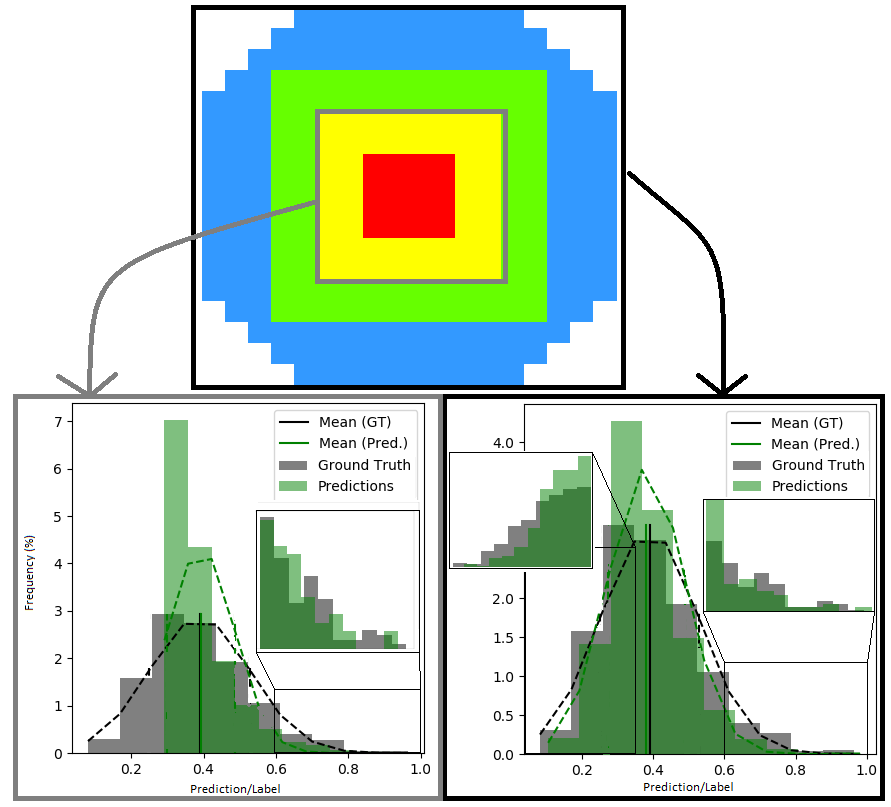
\includegraphics[scale=0.55]{Figures/region_compare2.png}
	\caption{Visual Summary of the Regional Feature Extraction Experiment} {\textbf{Top:} the concentric core regions as described in Figure~\ref{fig:regions} with two inclusive regions delineated which represent the features included in the models corresponding to the mid and bottom image. \textbf{Mid:} The distribution of predictions made by a model trained on features representing the central two regions (red and yellow in the image above). It can be seen that the distribution of predictions in the upper end of the histogram is similar to that of the ground truth. However, this model makes few predictions in the lower region of the distribution, effectively overestimating these results. \textbf{Bottom:} When including all regions in the feature set, superior model performance is seen. The shape of the distribution for the model predictions closely fits that of the ground truth. }
	\label{fig:central}
\end{figure*}

\subsection{Analysis and Discussion} \label{analysis}

Looking at the final model architecture 
(Figure~\ref{fig:model_architecture}), it can be seen that considerable complexity must be employed in terms of model parameters to produce the optimal result. This suggests that relationships between inputs and outputs are complex. This is to be expected, as the Parmec model is itself highly complex involving thousands of equations and parameters.
\\

\noindent
From Table~\ref{tab:encoding}, it can be seen that CNN architecture produces superior results to DNNs. Encoding the input features in a 3-dimensional format produces the best results. In addition, neural network models perform better than traditional methods as seen in Table~\ref{tab:traditional}. This suggests that true physical relationships within the data, i.e. local 3-dimensional configurations of cracks, have a causal relationship with displacements.
\\

\noindent
During the feature extraction experiment, it is noteworthy that the best result was achieved when including features representing all core regions, including the most distant, outer regions far removed from the location of the central channel. It was conjectured earlier that only the channels most local to the position of interest (the centre) would be of importance to predicting displacement. However, from Table~\ref{tab:regional} it can be seen that model performance drops sharply when excluding data for the main core channels. This suggests that cracking beyond the local region has a causal effect on the central channel's displacement. This phenomena is particularly interesting when considered along with the fact that the optimal convolutional window size is 3x3 (a relatively small window size by CNN standards) which suggests small patterns are most important.
\\

\noindent
Looking more closely at the results of this experiment, Figure~\ref{fig:central} shows the distribution of predictions made by models trained on the channels within the central core and full core. It can be seen that a model that excludes the main and greater core channels has difficulty making predictions in the lower part of the prediction spectrum. Perhaps the cracking status of bricks beyond the central core has some slackening or tightening effect on the centre of the core. The exact reason for this phenomenon will require further study.
\\

\noindent
Examining the results of the experiment which excludes features by core levels (Table~\ref{tab:levels}), it can be seen that the best overall result is achieved when including features for the top three levels (5~-~7). Note also that a similar performance is achieved with all arrangements except when only the top two levels were included (6~-~7), hence low sensitivity. From these results, we can conclude that the at least the top three levels have a discernible impact on the displacement of the central core channel.
\\

\noindent
Figure~\ref{fig:best_margins} shows the test predictions for the best performing model (3D CNN trained on features for levels 5-7) plotted against the ground truth. It can be seen that 94.8\% of the test predictions fall within a margin of 20\%  of the ground truth in absolute terms. Of the cases that fall outside this margin, we can see that most of them occur fairly close to the boundary. Using the same process as was used to generate this plot, we can identify the type of case which is difficult for the model to predict accurate values for, and generate cases accordingly. From a cursory examination of the cases outside of the 20\% margin from Figure~\ref{fig:best_margins}, it was observed that they contained on average 5\% fewer cracks in the top core level than the wider dataset. 
\\



\begin{figure}[h]
	\centering
	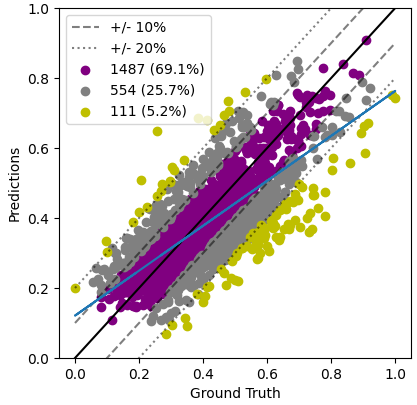
\includegraphics[scale=0.65]{Figures/best_results_distribution_margins.png}
	\caption{Model Predictions against Ground Truth for the Test Set} {A 'perfect' model would produce values on the solid black line i.e. exactly the ground truth values. Lines representing an error margin of 10 and 20 absolute percentage points of deviation can be seen. Data-points are coloured according to their deviation from the ground truth. The testing mean squared error for this model was 9e-3, with an mean absolute error of 7.4e-3. The blue line represents a linear fit with the equation 0.58x + 0.16. The $R^2$ value is 0.53. }
	\label{fig:best_margins}
\end{figure}

\begin{figure}[p]
	\centering
	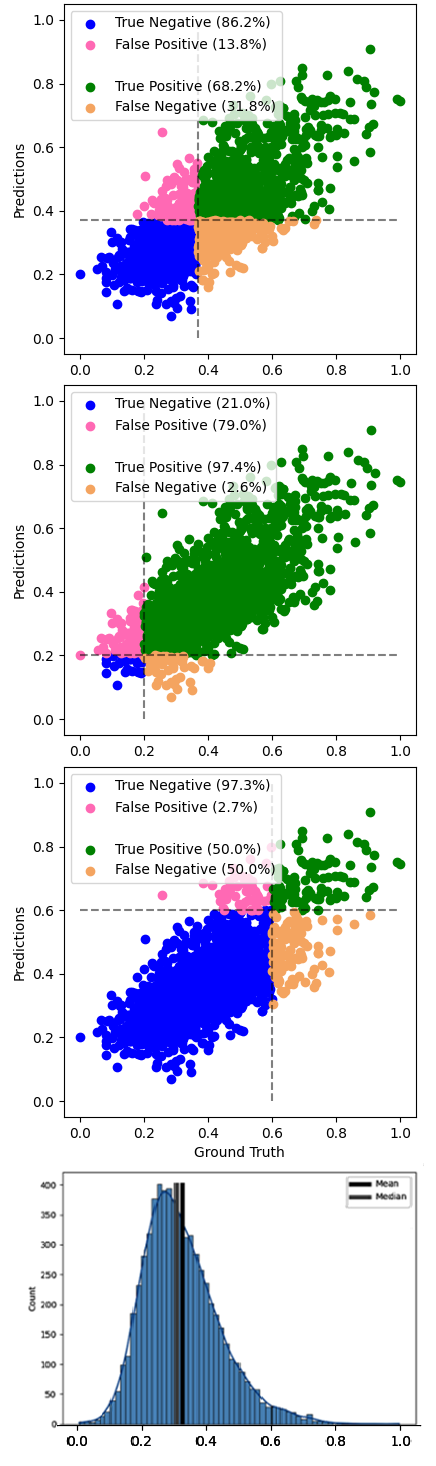
\includegraphics[scale=0.47]{Figures/best_results_analysis.png}
	\caption{Model Predictions against Ground Truth for the Test Set With Values Separated into Positives/Negatives by Three Different Thresholds} {The values are then classified by whether they fall into the same half of the distribution as the ground truth. \textbf{Top:} The separator is placed as the dataset mean (0.36). \textbf{Upper Middle:} The separator is placed to the lower side of the modal value. \textbf{Lower Middle:} The separator is placed just before a region of outlier values. \textbf{Bottom:} The dataset distribution for context.}
	\label{fig:best_analysis}
\end{figure}

\noindent
To further evaluate the performance of the model, we can separate the plot shown in Figure~\ref{fig:best_margins} into positive and negative values based on chosen thresholds. Figure~\ref{fig:best_analysis} shows the predictions and ground truth separated based on three chosen thresholds. Taking the mean as the positive/negative separator (top), it can be seen that the model performs well at predicting which region a given instance is in. However, the model performs less well at predicting values for cases at the very extremes of the data continuum (threshold of 0.2 and 0.6). Nevertheless, the 'false' examples are predicted as close to the boundary in all three graph configurations. In general, it can be seen that cases at the lower and upper ends of the data range are predicted as closer to the mean than the ground truth. Looking at the distribution of the dataset (bottom), a possible explanation is that it is highly 'biased' towards the region close to the mean i.e. the model has many fewer cases to learn from at the ends of the distribution.
\\

\noindent
Following the training process of all models discussed in this section, the generation of output values takes less than one second per instance. Using the same hardware, the equivalent data generation time would be over 2 hours using the original Parmec software.
\\

\noindent
To summarise the observations made:

\begin{enumerate}
	\item \textbf{Model Complexity:} the optimal surrogate model architecture exhibits considerable depth and width as well as requiring considerable refinement and tuning. This suggests a complex and non-trivial relationship between inputs and outputs.
	\item \textbf{Input Encoding:} optimal performance was seen when including true physical relationships in the input features i.e. a 3-dimensional encoding which represents the actual structure of the graphite core.
	\item \textbf{Feature Selection - Regional:} when selecting input features regionally by dividing the graphite core into radial segments, it was observed that optimal model performance was achieved when including data for all regions. This suggests that the cracking status of even bricks far away from the position of interest are important to the prediction of displacements. 
	
	\item \textbf{Feature Selection - Level:} when selecting input features vertically by selecting inputs from inclusive ranges of core levels, it was observed that optimal model performance was achieved when including data for the top five levels. Further, little performance sensitivity was observed when reducing the levels included in the feature dataset.
	
	\item \textbf{Difficult to Predict Cases: } cases were identified that are difficult for the model to accurately predict. Through examining these cases, some common characteristics were observed. These observations may help to design further machine learning experiments or inform engineering analysis.
	\item \textbf{Dataset Bias:} we can note that the model has lower prediction accuracy near the extremes of the data range. This can be explained by the fact that the dataset is biased towards the central region, meaning the model has fewer examples from the extremes to learn from.
\end{enumerate}


\section{Conclusion} \label{conclusion}

A surrogate machine learning model was developed which aims to predict seismic graphite core displacements from crack configurations for the advanced gas-cooled reactor. The model was trained on a dataset generated by a software package which simulates the behaviour of the graphite core during a severe earthquake. 
\\

\noindent
The main motivation behind this research was to increase the computational efficiency of seismic displacement output data generation in order to allow a wider search of the vast problem space. Following the training process of the models, the generation of output values takes less than one second. Using the same hardware, the equivalent data generation time would be over 2 hours using the original Parmec software.
\\

\noindent
The best performing model was capable of making 95\% of test set predictions within a 20 percentage point margin of the ground truth. Although this result demonstrates progress towards the development of an efficient and accurate machine learning surrogate, the high standards within the nuclear safety field mean that it is unlikely to be at a stage were it could be commercially deployed. Nevertheless, machine learning techniques were identified as highly applicable to this particular problem. For example, Convolutional neural networks were identified as more effective than other techniques available. Additionally insights into optimal hyper-parameters and inputs were also garnered. These observations may guide and support further development and progress in this area.



    
